\chapter{Performance Pay in Education}

\fancyhead[L]{ECON0024}
\fancyhead[C]{Ch.10 Performance Pay in Education}
\fancyhead[R]{Xiaotian Tian}
\fancyfoot[L]{\hyperlink{tableofcontents}{Back to Table of Contents}}
\fancyfoot[R]{Xiaotian Tian}

\section{Motivation}

    School resources may have limited effectiveness because schools do not face market incentives. Thus, maybe we can introduce some market incentives:
    \begin{itemize}
        \item School choice (allowing parents to choose schools)
        \item Incentives in schools (for teachers/students)
    \end{itemize}
    We will focus on the second one in this lecture.
    
    In reality, designing incentives for teachers is complicated due to the multitasking problem introduced below.

\section{$\star$ Model of Multitasking (\cite{neal_chapter_2011})}
    
    We want to elicit effort from teachers. Specifically, we need to address two main issues:
    \begin{itemize}
        \item \emphb{Multitasking} -- there are several activities a teacher undertakes
        \item \emphb{Unobservable outputs} -- It is hard to measure performance
    \end{itemize}
    
    \subsection{Setup}
        
        \subsubsection{Basics}
            
            The education authority hires 1 teacher to teach 1 student.
            
            The teacher allocates time/effort to two different tasks: $t_1$ and $t_2$ are time spent on each task.
        
        \subsubsection{Human Capital Production}
        
            \begin{equation*}
                h = f_1t_1 + f_2t_2 + e
            \end{equation*}
            where:
            \begin{itemize}
                \item $h$: human capital measured in \pounds
                \item $t_1$ and $t_2$: teacher's time spent on each task
                \item $f_1,f_2$: constants
                \item $e$: random shock with mean zero and independent of $t_1,t_2$
                \item $h-e$ is the result of teacher efforts, over which the teacher has control
            \end{itemize}
            
        \subsubsection{Observable Performance}
        
            The education authority cannot observe $h,t_1,t_2$.
            
            Only a statistical measure of teacher performance $p$ is observed (e.g. a test score):
            \begin{equation}
                p = g_1t_1 + g_2t_2 + v
                \label{eqn:edu_performance}
            \end{equation}
            where:
            \begin{itemize}
                \item $t_1$ and $t_2$: teacher's time spent on each task
                \item $g_1,g_2$: constants
                \item $v$: random shock with mean zero and independent of $e,t_1,t_2$
            \end{itemize}
            
        \subsubsection{Teacher's Wage and Utility}
        
            \emphb{Wage}:
            \begin{equation*}
                w = s+ bp
            \end{equation*}
            where:
            \begin{itemize}
                \item $s$: base salary
                \item $b$: bonus for performance
                \item $p$: student's performance (equation \ref{eqn:edu_performance})
            \end{itemize}
            
            \emphb{Utility}:
            \begin{equation*}
                U = \underbrace{E[s+bp]}_{=E[w]=X} - \underbrace{\left[ \frac{1}{2}(t_1-\overline{t_1})^2 + \frac{1}{2}t_2^2 \right]}_{C(t_1,t_2)}
            \end{equation*}
            where:
            \begin{itemize}
                \item $X=E[w]=E[s+bp]$: teacher's expected income
                \item $C(t_1,t_2) = frac{1}{2}(t_1-\overline{t_1})^2 + \frac{1}{2}t_2^2$: teacher's cost of effort
                \begin{itemize}
                    \item $\overline{t_1}$: the minimal amount of effort spent on task 1 (e.g. showing up)
                    \item $C(t_1,t_2)$ is increasing in both $t_1,t_2$
                \end{itemize}
            \end{itemize}
            
            We also have an outside option for the teacher with utility $U_0$.
            
        \subsubsection{Education Authority's Target Function}
        
            Suppose the education authority is a benevolent social planner who maximises:
            \begin{maxi}|s|{t_1,t_2}{E(h)-C(t_1,t_2)}{\label{eqn:edu_opt1}}{}
                \addConstraint{h}{=f_1t_1 + f_2t_2 + e}
                \addConstraint{C(t_1,t_2)}{=\frac{1}{2}(t_1-\overline{t_1})^2 + \frac{1}{2}t_2^2}
            \end{maxi}

    \subsection{Ideal Optimisation (If All Observable)}
        
        If all variables are observable, the education authority can solve the optimisation \ref{eqn:edu_opt1} directly:
        \begin{equation*}
            \implies \max_{t_1,t_2} f_1t_1 + f_2t_2 - \left[ \frac{1}{2}(t_1-\overline{t_1})^2+\frac{1}{2}t_2^2 \right]
        \end{equation*}
        First order conditions:
        \begin{equation*}
            \begin{cases}
                    f_1 - \frac{1}{2} 2(t_1 - \overline{t_1}) &= 0\\
                    f_2 - \frac{1}{2} 2t_2 &= 0
            \end{cases}
        \end{equation*}
        \emphb{Optimum with perfect information}:
        \begin{equation*}
            \color{Red}
            \begin{cases}
                t_1^* &= f_1 + \overline{t_1}\\
                t_2^* &= f_2
            \end{cases}
        \end{equation*}
        However, this is not feasible in reality because $t_1,t_2$ are unobservable.
    
    \subsection{Optimisation If Only Observe Scores}
    
        In reality, the educational authority only observe a performance score $p$ (equatin \ref{eqn:edu_performance}). Similar to any typical mechanism design problem with moral hazard, we work backwards by solving teacher's optimisation first.
        
        \subsubsection{Step 1: Teacher's Optimisation}
        
            Given a level of incentive ($b$), the teacher's optimal choice of $t_1,t_2$:

            \begin{align*}
                \max_{t_1,t_2} E[U] &= \underbrace{E[s+bp]}_{=E[w]} - \underbrace{\left[ \frac{1}{2}(t_1-\overline{t_1})^2 + \frac{1}{2}t_2^2 \right]}_{C(t_1,t_2)}\\
                &= s + b(g_1t_1 + g_2t_2) - \left[ \frac{1}{2}(t_1-\overline{t_1})^2 + \frac{1}{2}t_2^2 \right]
            \end{align*}
            \emphb{First order conditions for teachers}:
            \begin{equation}
                \begin{cases}
                    t_1 &= bg_1 + \overline{t_1} \\
                    t_2 &= bg_2
                \end{cases}
                \label{eqn:edu_teacher_opt}
            \end{equation}
            We can see that $b\uparrow \implies t_1\uparrow, t_2\uparrow$.
            
        \subsubsection{Step 2: Educational Authority's Optimisation}
        
            Given the teacher's response (equation \ref{eqn:edu_teacher_opt}), the educational authority's optimisation becomes:
            \begin{maxi}|s|{b}{E(h)-C(t_1,t_2)= f_1t_1 + f_2t_2 - \left[ \frac{1}{2}(t_1-\overline{t_1})^2+\frac{1}{2}t_2^2 \right]}{\label{eqn:edu_auth_opt}}{}
                \addConstraint{t_1}{=bg_1+\overline{t_1}}
                \addConstraint{t_2}{=bg_2}
            \end{maxi}
            Solving the constrained optimisation above, we can get the \emphb{optimal choice of incentive}:
            \begin{equation*}
                \color{red} b^* = \frac{f_1g_1 + f_2g_2}{g_1^2 + g_2^2}
            \end{equation*}
            \begin{itemize}
                \item $b>0$ as long as $f_1g_1 + f_2g_2 > 0$
                \item $b=0$ if $f_2=0$ and $g_1=0$ \\
                i.e. \emph{no incentive} if $t_2$ is not productive and $t_1$ is not reflected in the test
                \item $b=1$ if $f_1=g_1,f_2=g_2$\\
                i.e. \emph{full incentive} if the sensitivity of test scores is the same as the sensitivity of human capital
                \item $f_1g_2, f_2g_2$ are substitutes (they both lead to higher bonus)
                \begin{itemize}
                    \item $f_1$ and $g_1$ raise the effect of each other on $b$, so they are complements
                    \item $f_2$ and $g_2$ raise the effect of each other on $b$, so they are complements
                \end{itemize}
            \end{itemize}
            Then, the \emphb{overall optimal choice of teachers} is:
            \begin{equation*}
                \color{red}
                \begin{cases}
                    t_1^* &= \frac{f_1g_1^2+f_2g_1g_2}{g_1^2+g_2^2} + \overline{t_1} \\
                    t_2^* &= \frac{f_1g_1g_2 + f_2g_2^2}{g_1^2+g_2^2}
                \end{cases}
            \end{equation*}
            This is not the most efficient solution where we have perfect information, unless $f_1=g_1,f_2=g_2$. However, this is the best outcome achievable.

            The educational authority should design the test to make $p$ as close to $h$ as possible.

    \subsection{Use Value-Added (VA) instead of Raw Score}

        In its simplest form, VA is measured as:
        \begin{equation*}
            VA = T_1 - T_0
        \end{equation*}
        where:
        \begin{itemize}
            \item $T_0$: beginning of year test score
            \item $T_1$: end of year test score
        \end{itemize}
        VA measures the learning during the year.

        It is better (more accurate) than using $T_1$ along, because it accounts for the different starting point of students. 

        However, simply using $T_1-T_0$ may not be a good measure of learning. We could also use more complex measures of VA, such as $\frac{T_1}{T_0}$ or controlling for other student characteristics.
        
    \subsection{Common Problems of Cardinal Performance Pay}

        \subsubsection{Teaching to the Test}

            Teachers respond to incentives. This issues is especially serious when we are far away from $f_1=g_1$ and $f_2=g_2$ (poor test design).

            Meanwhile, we cannot simply change the test items frequently to avoid the problem, because we need assessments to be comparable over time.

        \subsubsection{Corruption/Cheating}

            Teachers may manipulate which students show up for testing. \cite{jacob_rotten_2003} shows that around 5\% of the classrooms in Chicago's public school system have this issue.
        

\section{Relative Performance Pay}

    \subsection{Overview}

        One of the most important problem of the cardinal performance pay system we discussed above is that \emph{test scores do not have a scale}.

        One alternative is to pay teachers based on an \emphb{ordinal measure of performance}, such \emphb{tournaments} between teachers. This is especially useful when observing absolute performance is difficult, but ranking is easy.

        Specifically, the educational authority offers a fixed pot of money, which will be paid to workers based on their relative performance. In this case, some will win while some will lose.

        The \emphb{advantages} of relative performance pay are:
        \begin{itemize}
            \item It's harder to corrupt.\\
            For example, even if all teachers collude to exercise low effort, there is a strong incentive to deviate and get the prize.
            \item No longer need to have similar assessments over time, limiting teaching to the test
        \end{itemize}

    \subsection{Pay for Percentile (\cite{barlevy_pay_2012}) -- Best in Theory}

        \cite{barlevy_pay_2012} designs a "pay for percentile" system, and demonstrates that such a system can elicit \empha{efficient effort from all teachers in all classrooms}.

        Specific procedures:
        \begin{itemize}
            \item For each student is a school system, first form a comparison set of students against which the student will be compared (the general idea is to form a set that contains all other students in the system who begin at the same level of baseline achievement in a comparable classroom setting)
            \item At the end of the year, give an assessment to all students.
            \item Assign each student to a percentile score based on his end-of-year ranking among the students in his comparison set
            \item For each teacher, sum these within-peer percentile scores over all the students she teaches and denote this sum as a percentile performance index
            \item Pay each teacher a common base salary plus a bonus that is proportional to her percentile performance index
        \end{itemize}

\section{Evidences on Performance Pay}

    \subsubsection{Overview}

        Most studies find performance pay useful.

        \begin{figure}[H]
            \centering
            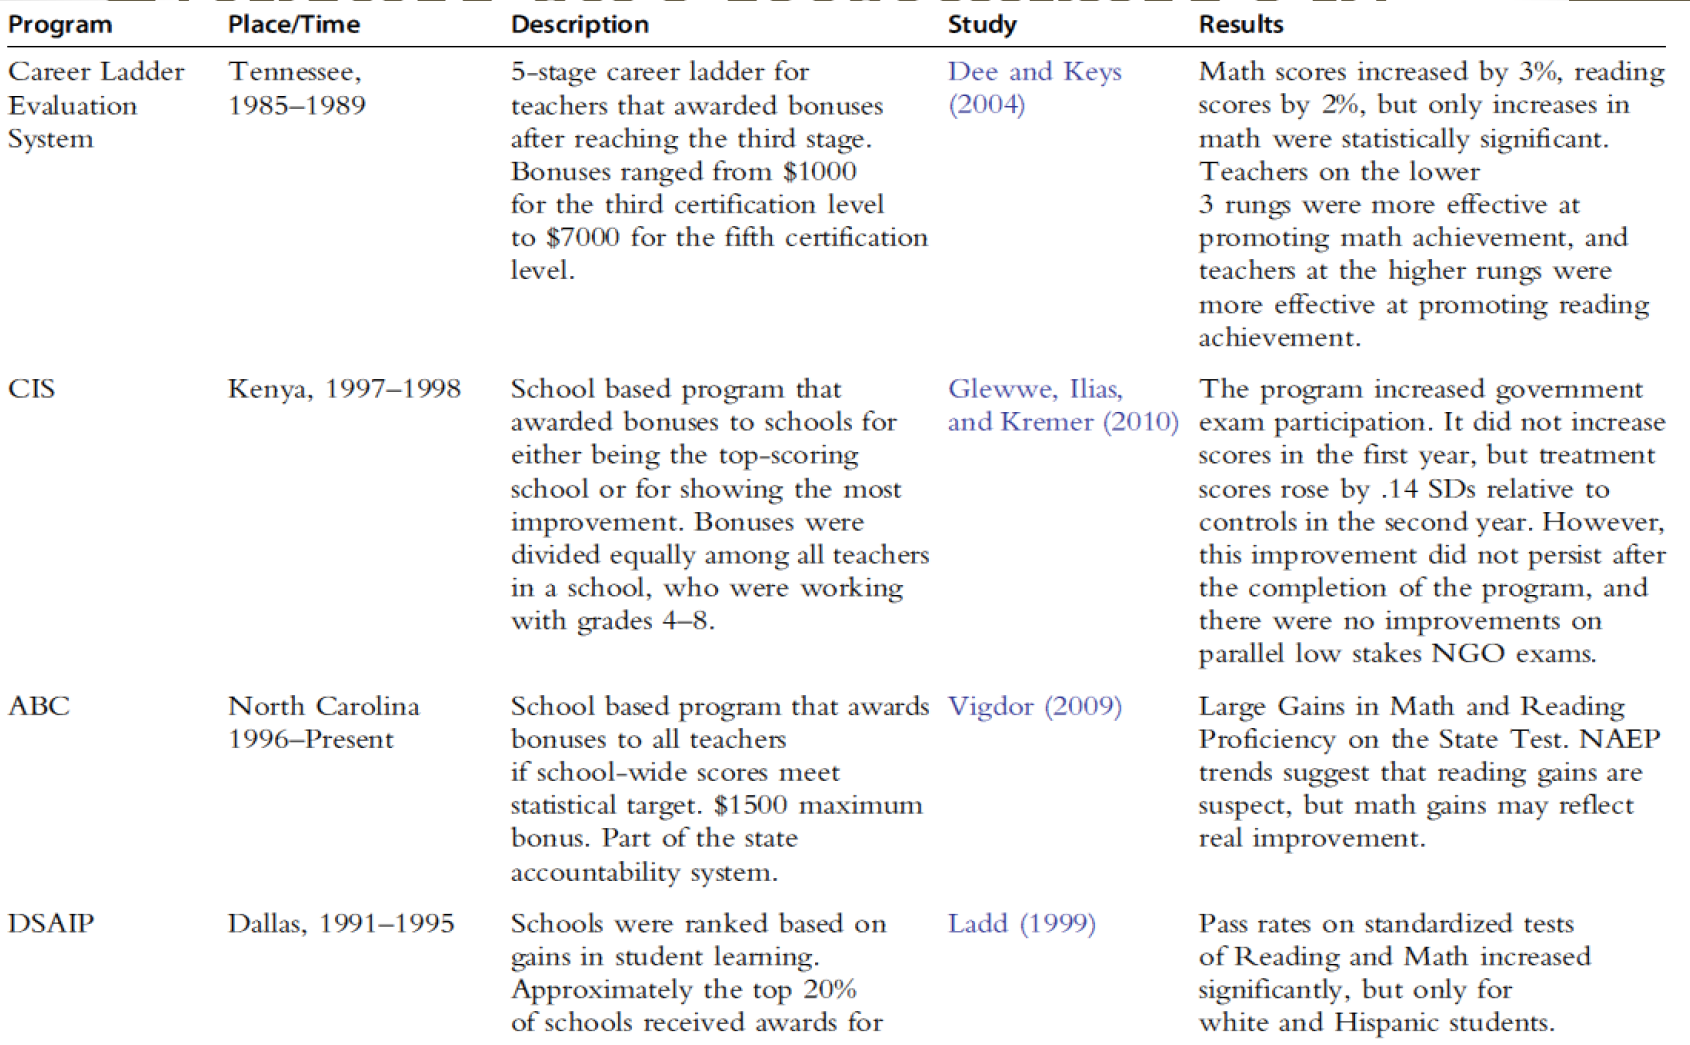
\includegraphics[width=4.5in]{images/ch10/10 pp 1.png}
            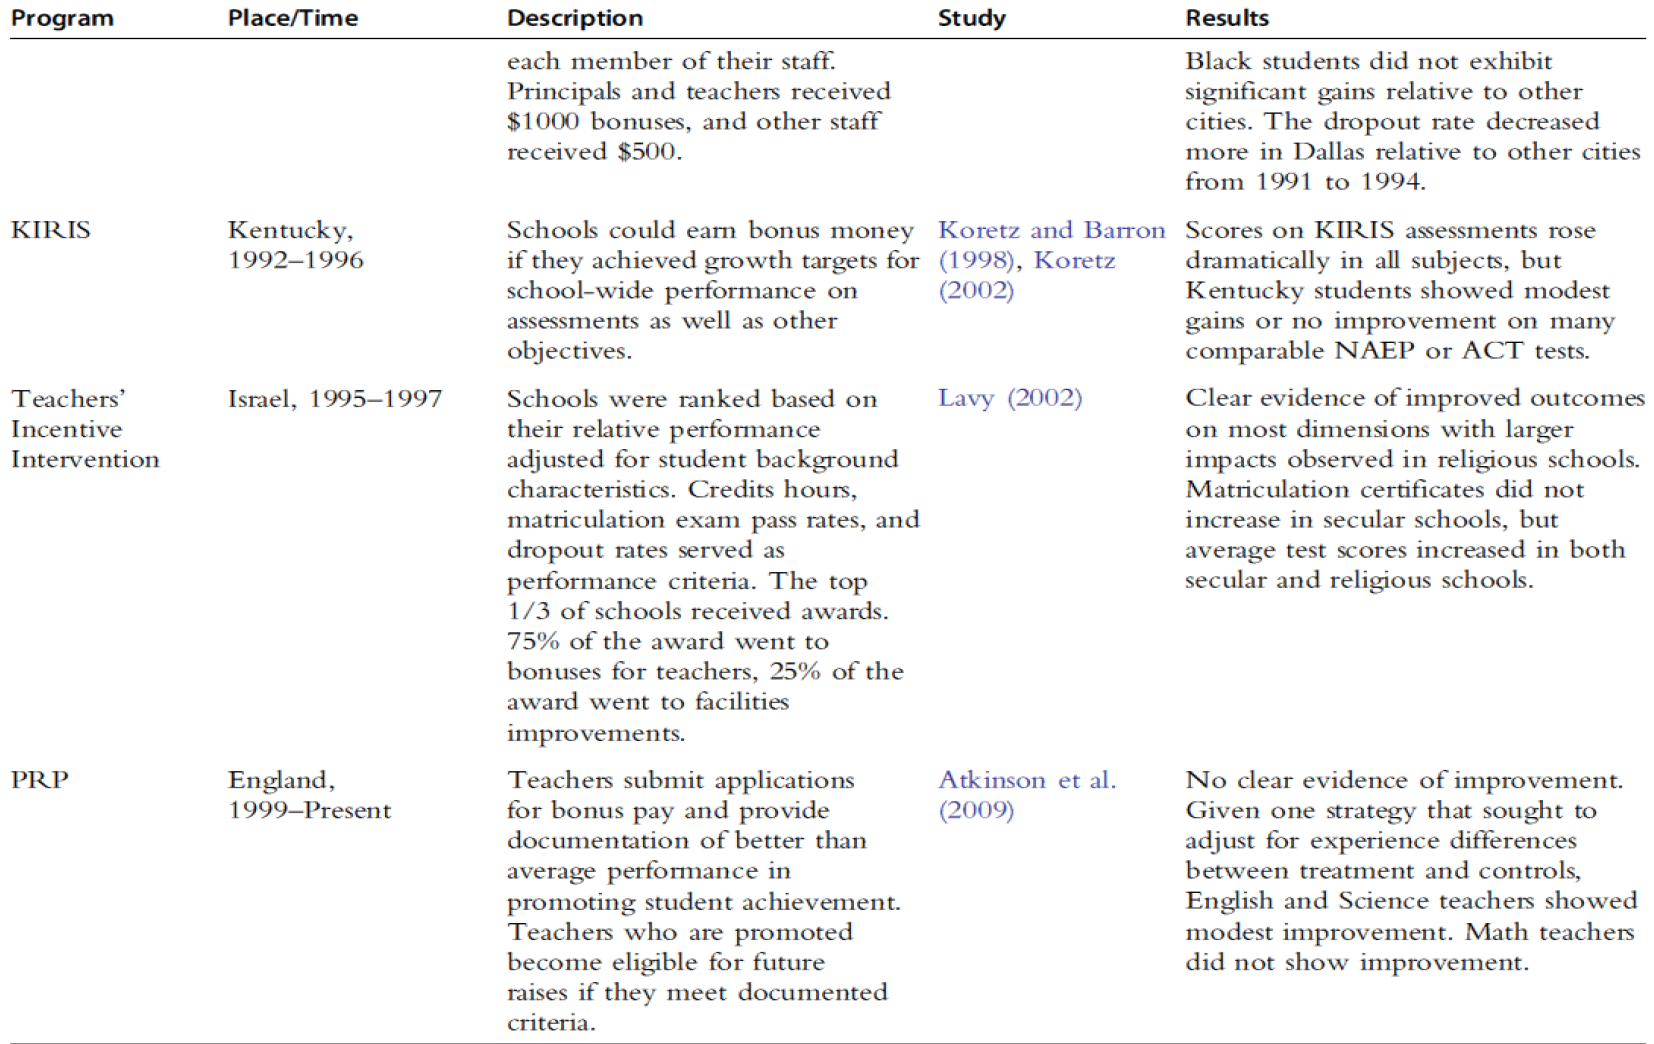
\includegraphics[width=4.5in]{images/ch10/10 pp 2.png}
        \end{figure}
        \begin{figure}[H]
            \centering
            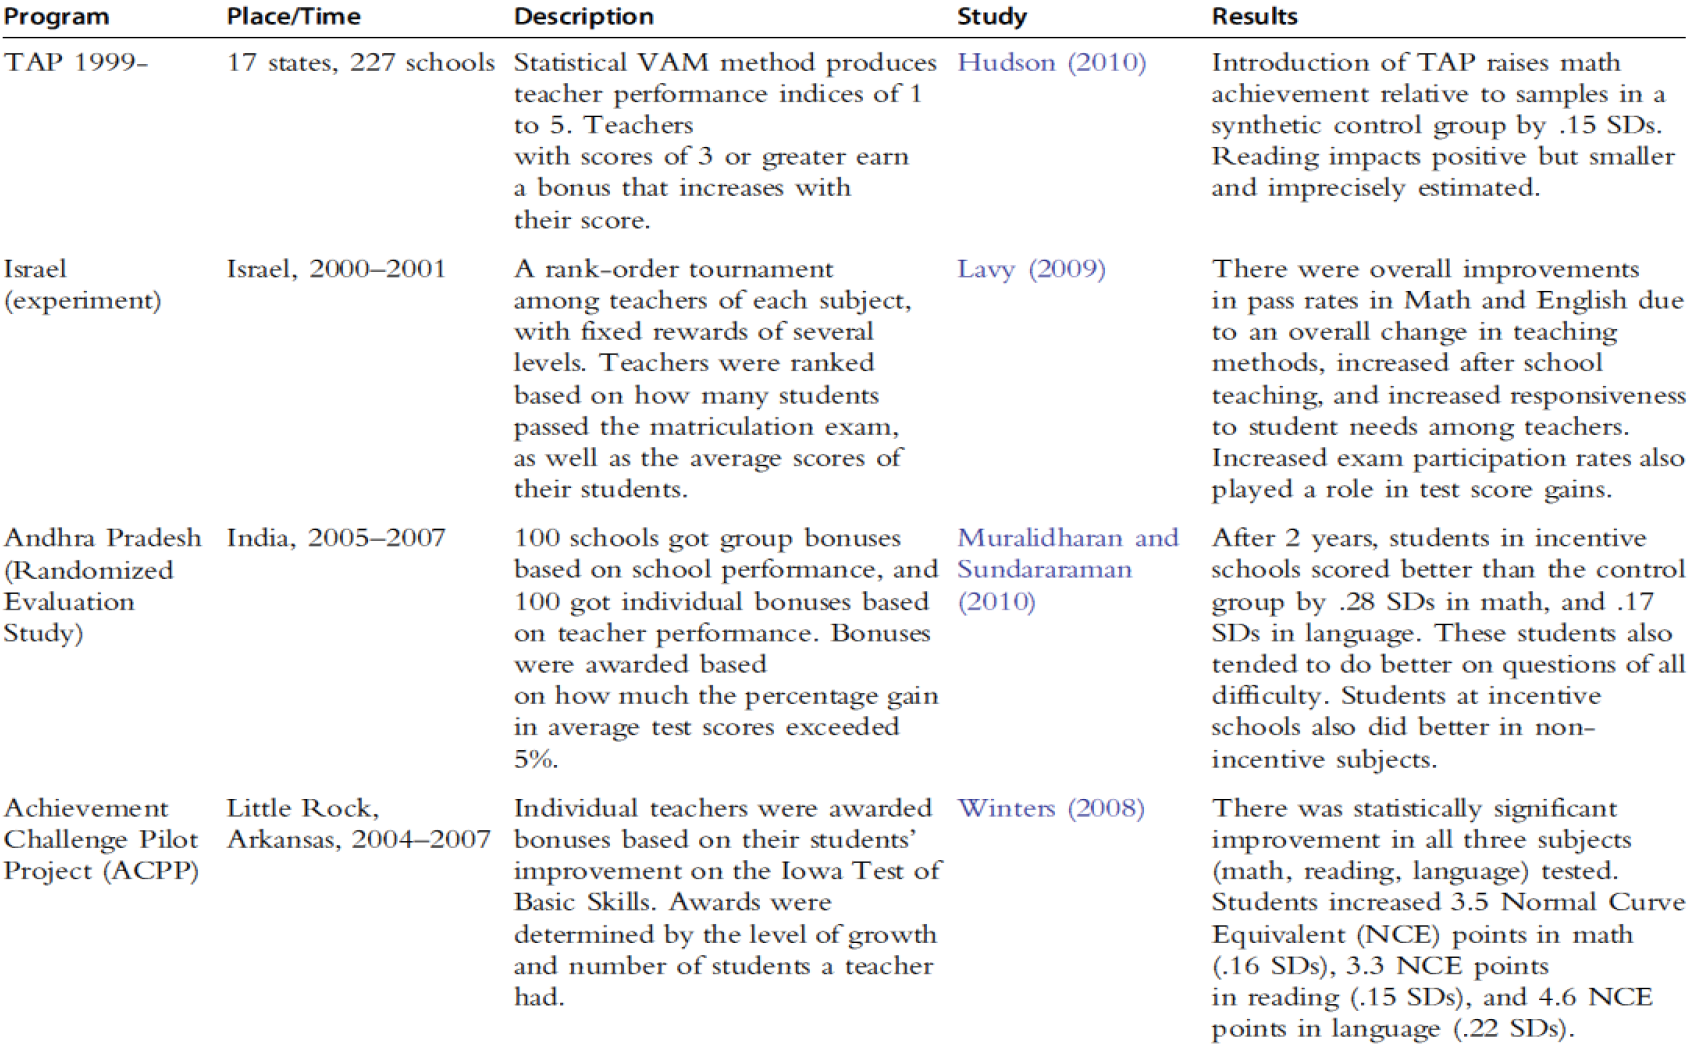
\includegraphics[width=4.5in]{images/ch10/10 pp 3.png}
            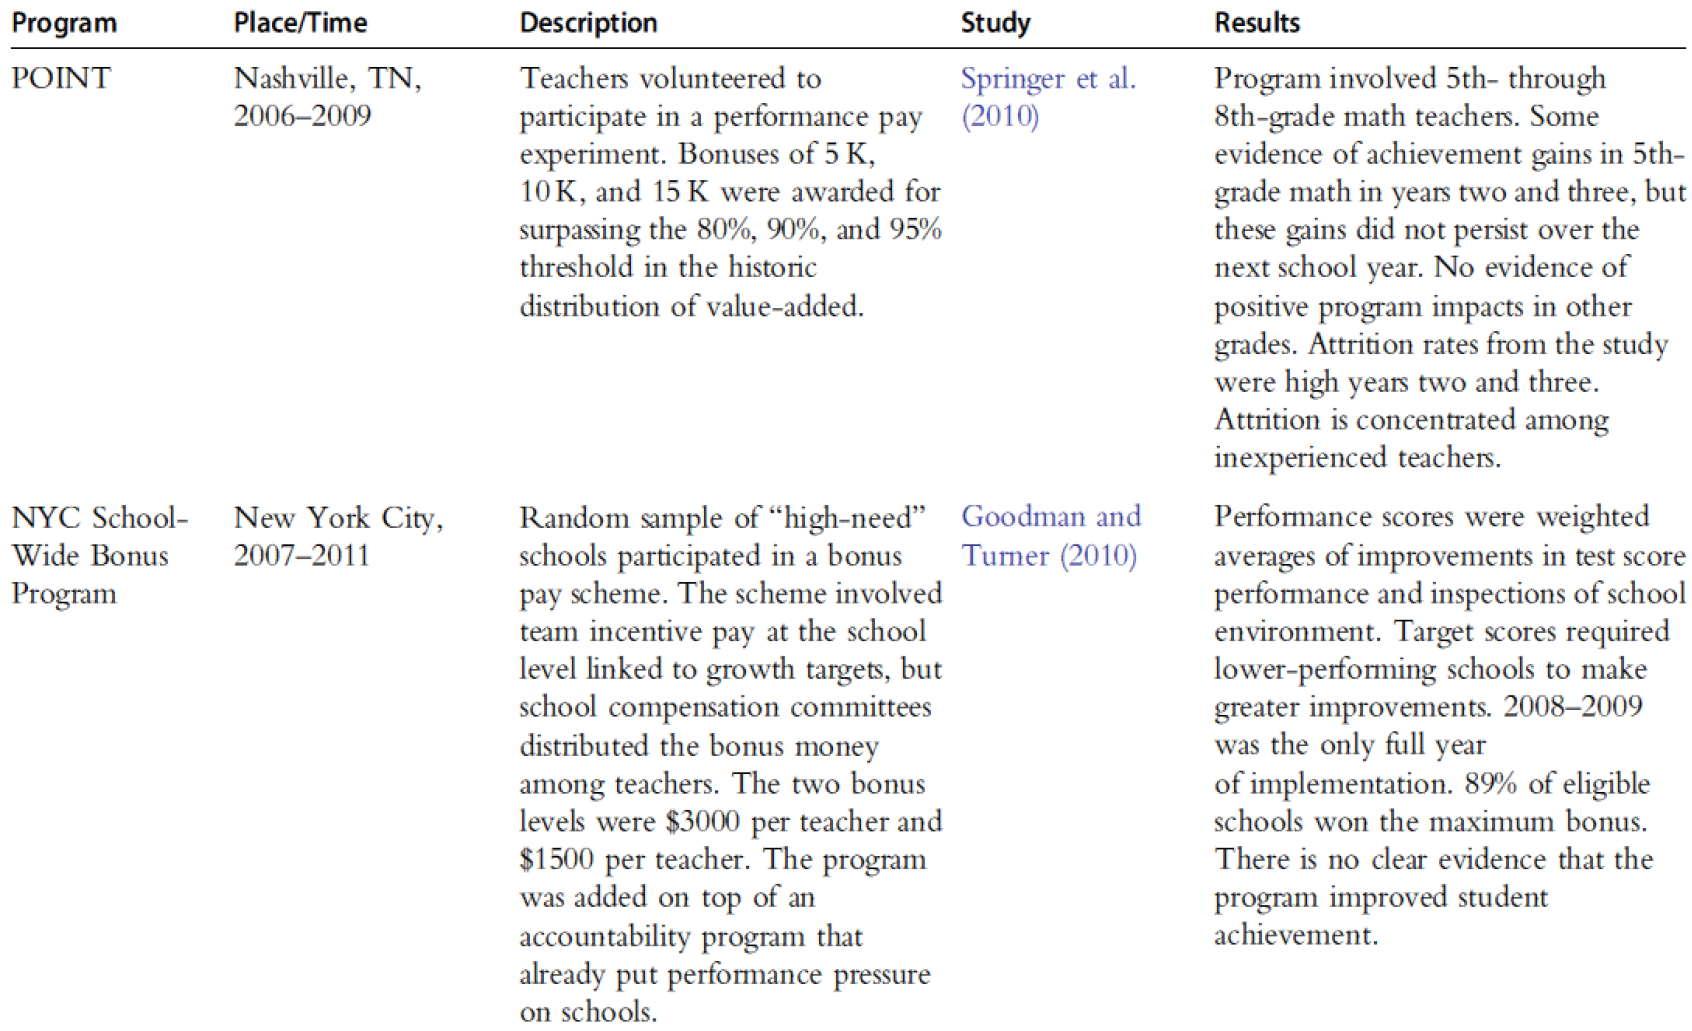
\includegraphics[width=4.5in]{images/ch10/10 pp 4.png}
            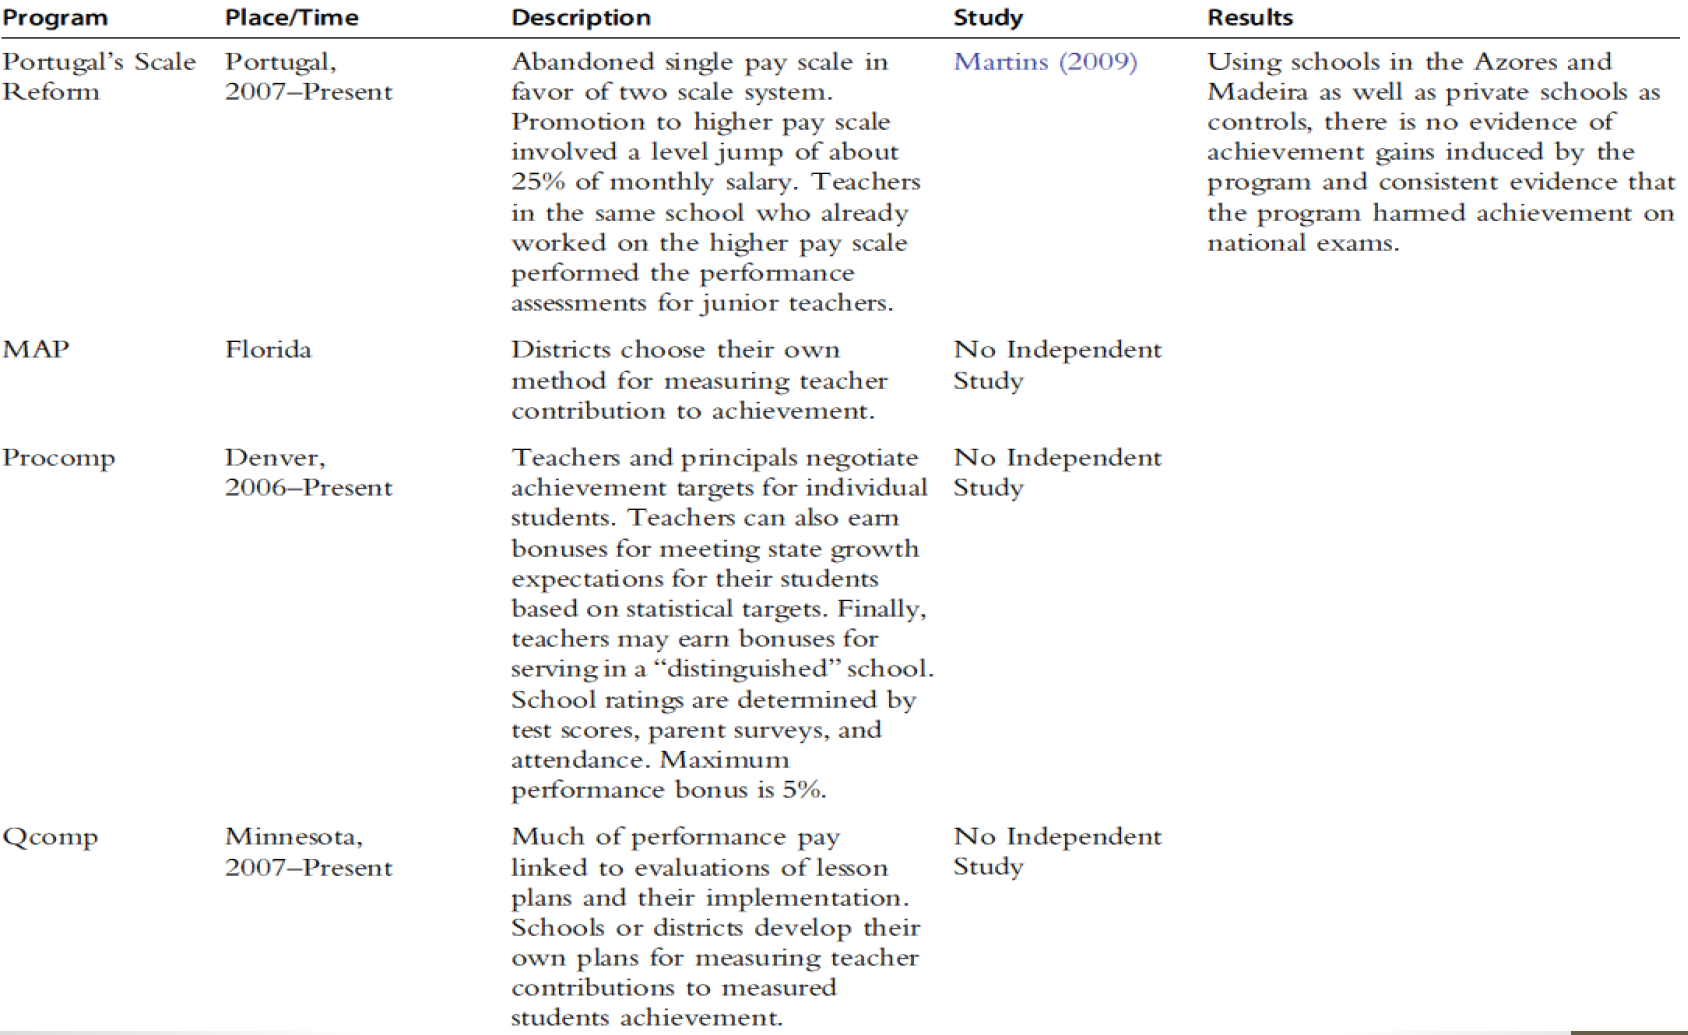
\includegraphics[width=4.5in]{images/ch10/10 pp 5.png}
        \end{figure}

    \subsection{2 Specific Papers on Cardinal Performance Pay}
        \subsubsection{\cite{muralidharan_teacher_2011}}

            \cite{muralidharan_teacher_2011} run RCTs in elementary schools in India with individual and group incentives (3\% of average pay). Results show significant improvements.
            \begin{figure}[H]
                \centering
                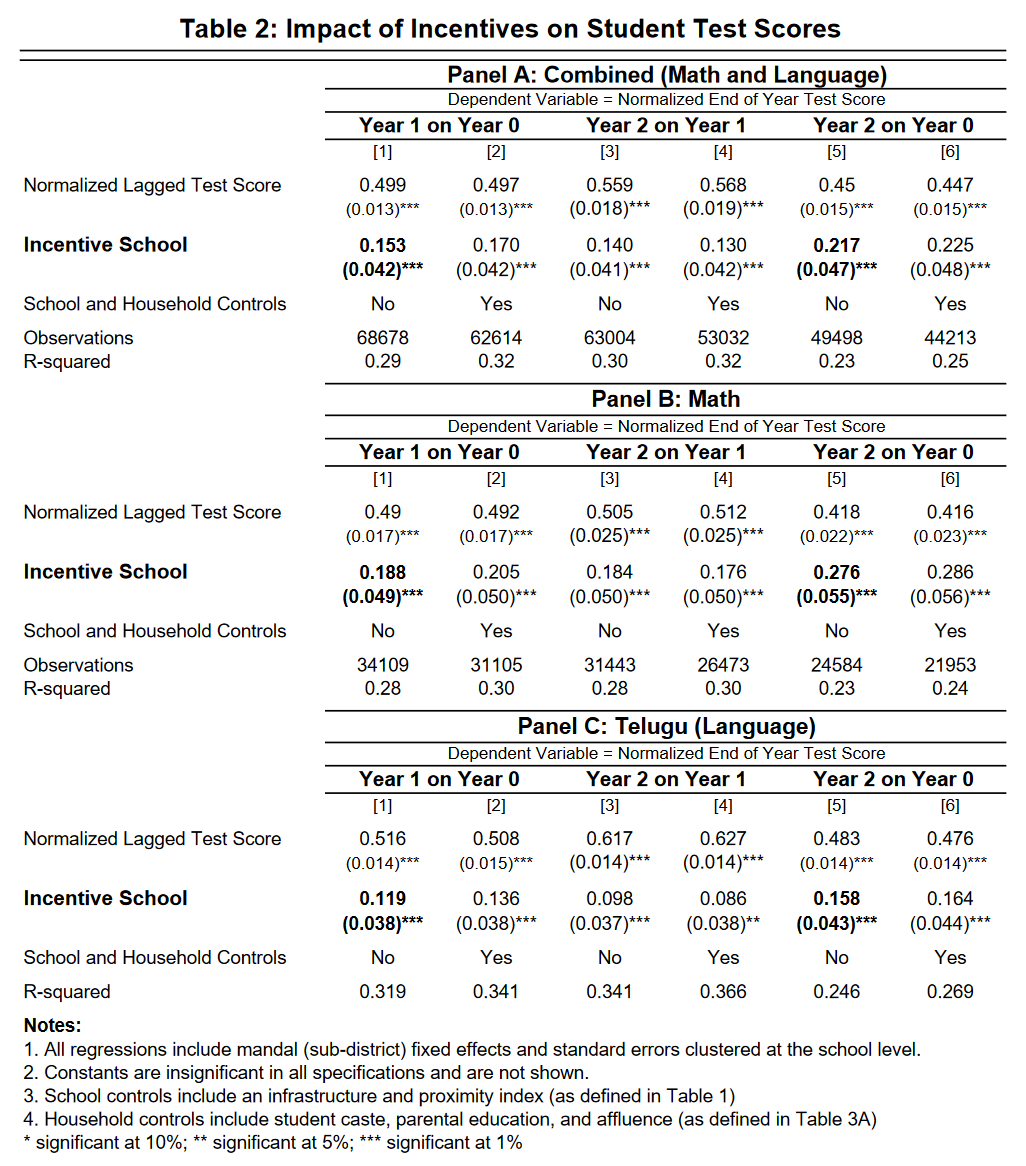
\includegraphics[width=4.5in]{images/ch10/10 muralidharan 1.png}
                \caption{Outcomes (\cite{muralidharan_teacher_2011})}
            \end{figure}
            \begin{figure}[H]
                \centering
                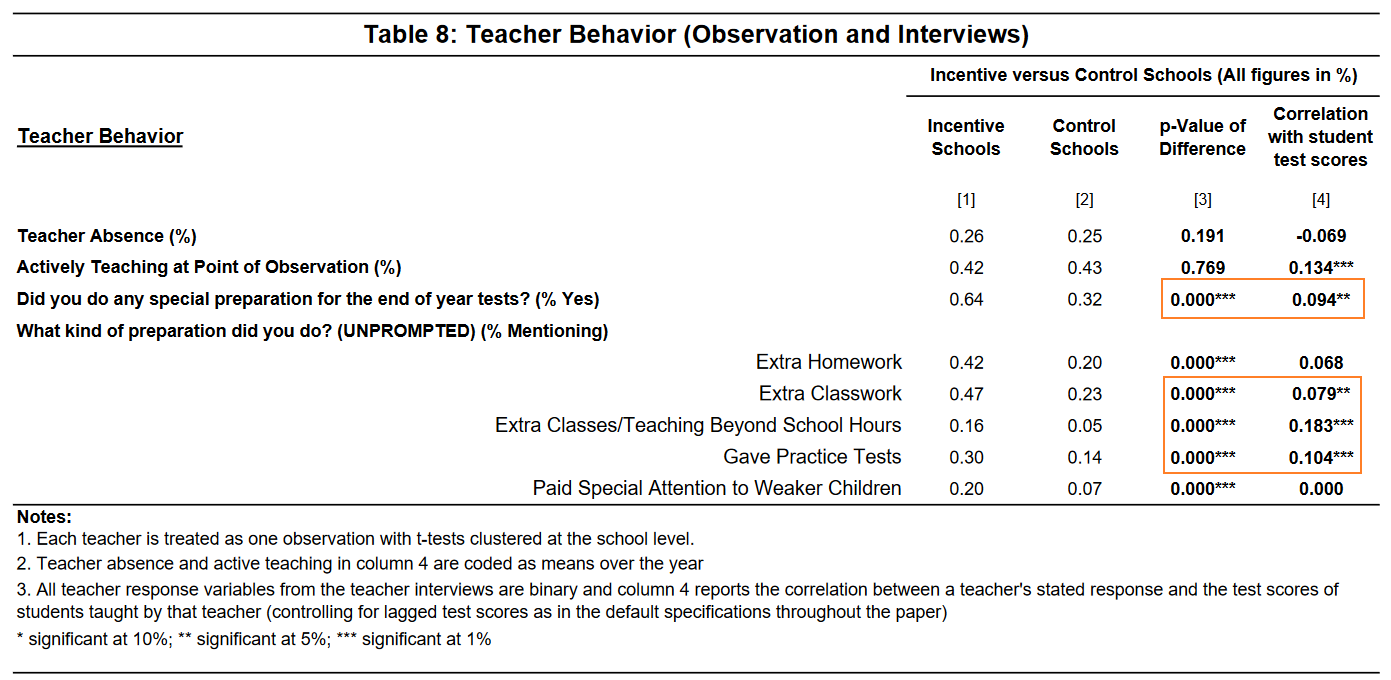
\includegraphics[width=5in]{images/ch10/10 muralidharan 2.png}
                \caption{Channels (\cite{muralidharan_teacher_2011})}
            \end{figure}
        \subsubsection{\cite{behrman_aligning_2015}}

            \cite{behrman_aligning_2015} conduct RCTs in secondary schools in Mexico. There are three treatment groups: a group where students get bonus, a group where teacher get bonus, and a group where everyone get bonus.
            \begin{figure}[H]
                \centering
                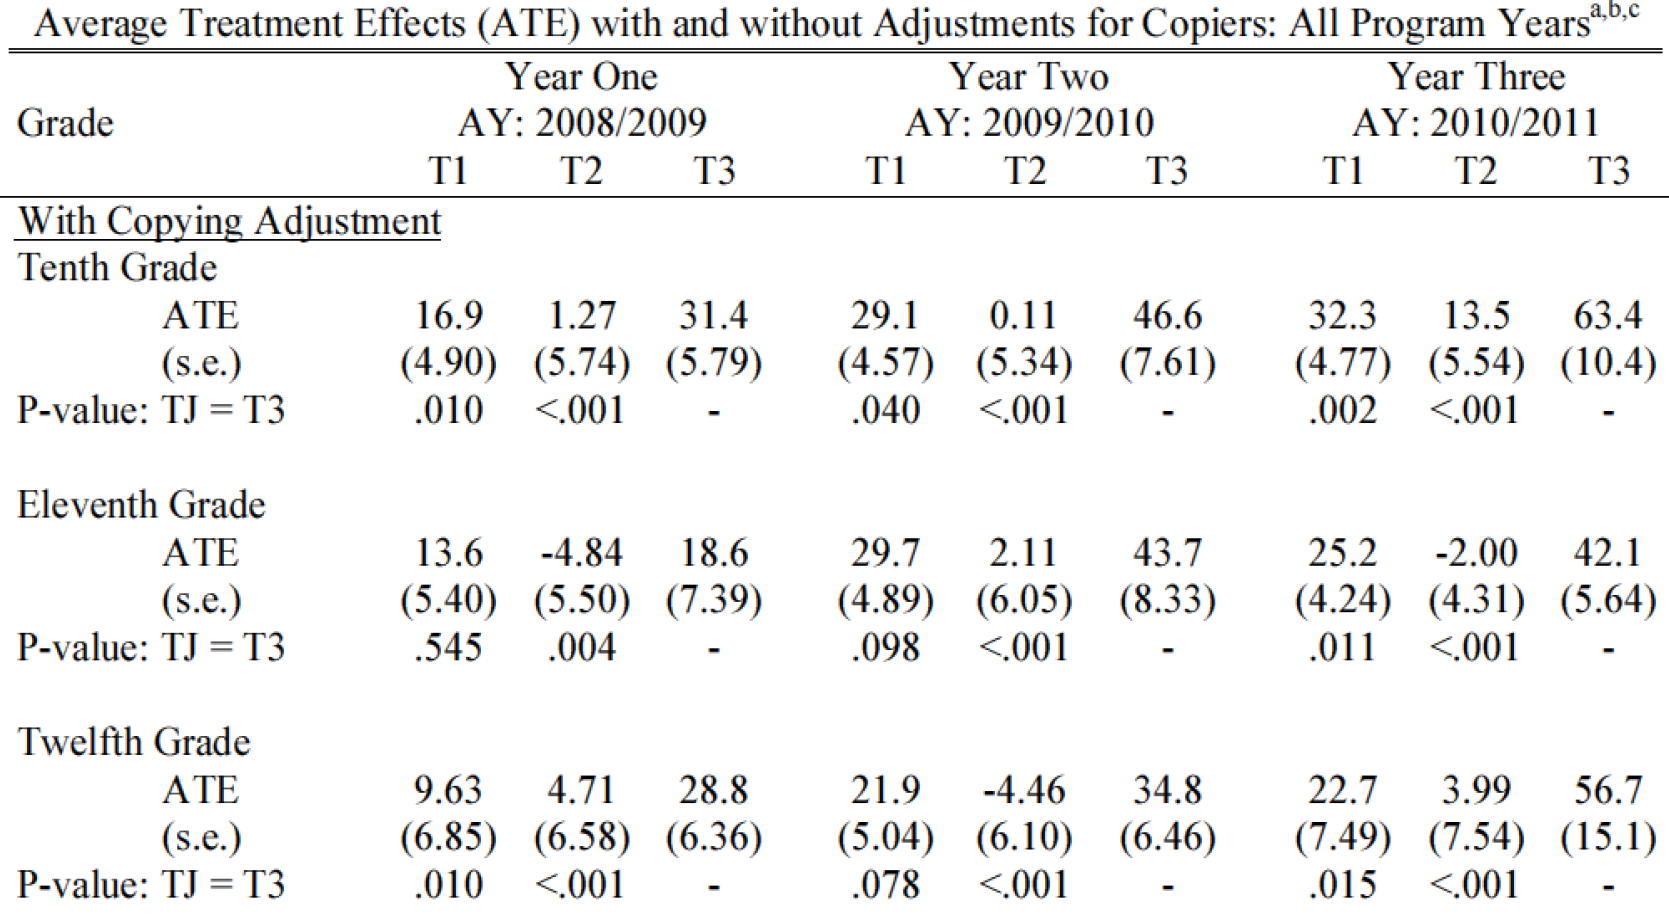
\includegraphics[width=4.5in]{images/ch10/10 berhman 1.png}
                \caption{Outcomes (\cite{behrman_aligning_2015})}
            \end{figure}
            Their results are adjusted for potential cheating. Giving everyone the bonus turns out to be the most effective, and the effect increases by time.
            \begin{figure}[H]
                \centering
                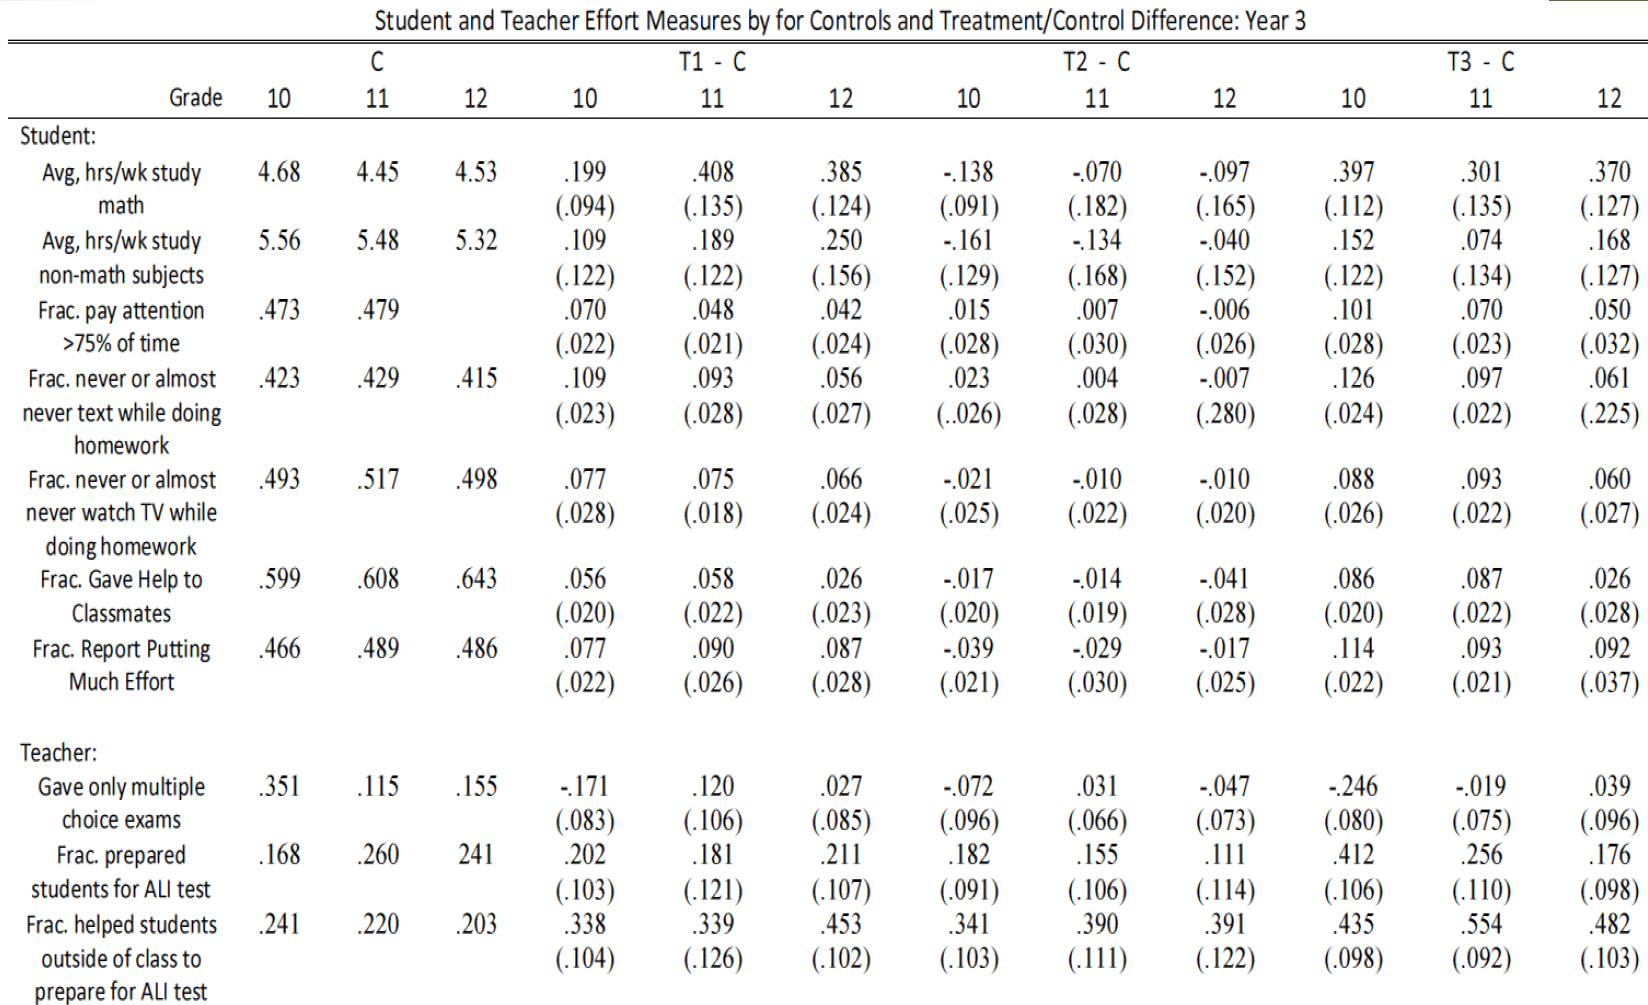
\includegraphics[width=4.5in]{images/ch10/10 berhman 2.png}
                \caption{Channels (\cite{behrman_aligning_2015})}
            \end{figure}

    \subsection{1 Paper on Relative Performance Pay}

        \cite{lavy_performance_2009} analyses the effect of a tournament which is based on performance relative to other teachers in the same subject. (Also a RCT.)
        \begin{figure}[H]
            \centering
            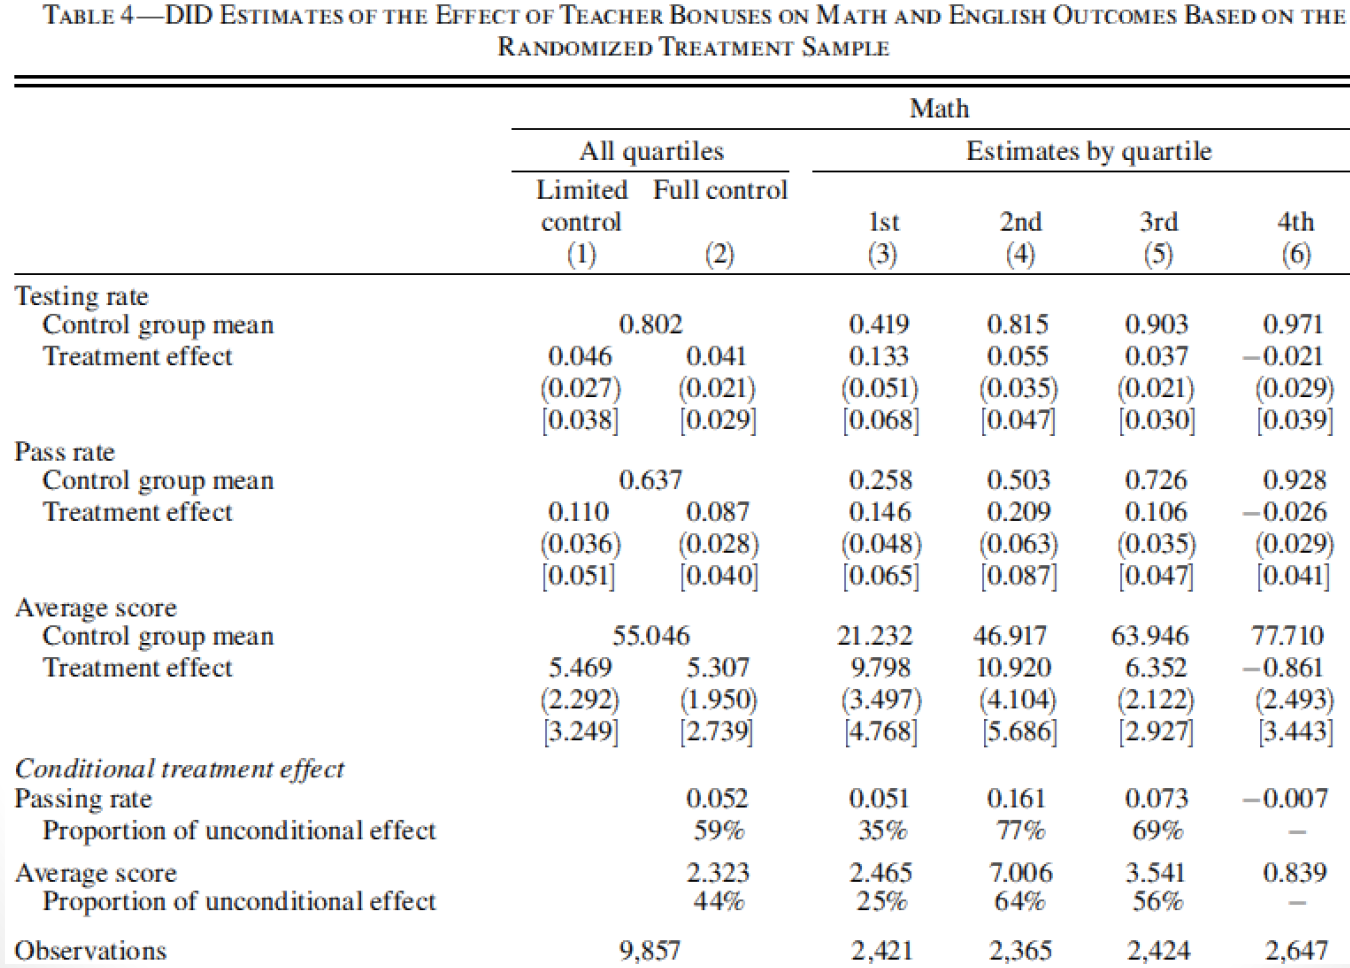
\includegraphics[width=4.5in]{images/ch10/10 lavy 1.png}
            \caption{Outcomes (\cite{lavy_performance_2009})}
        \end{figure}
        The outcome improves the most in the lower half.
        \begin{figure}[H]
            \centering
            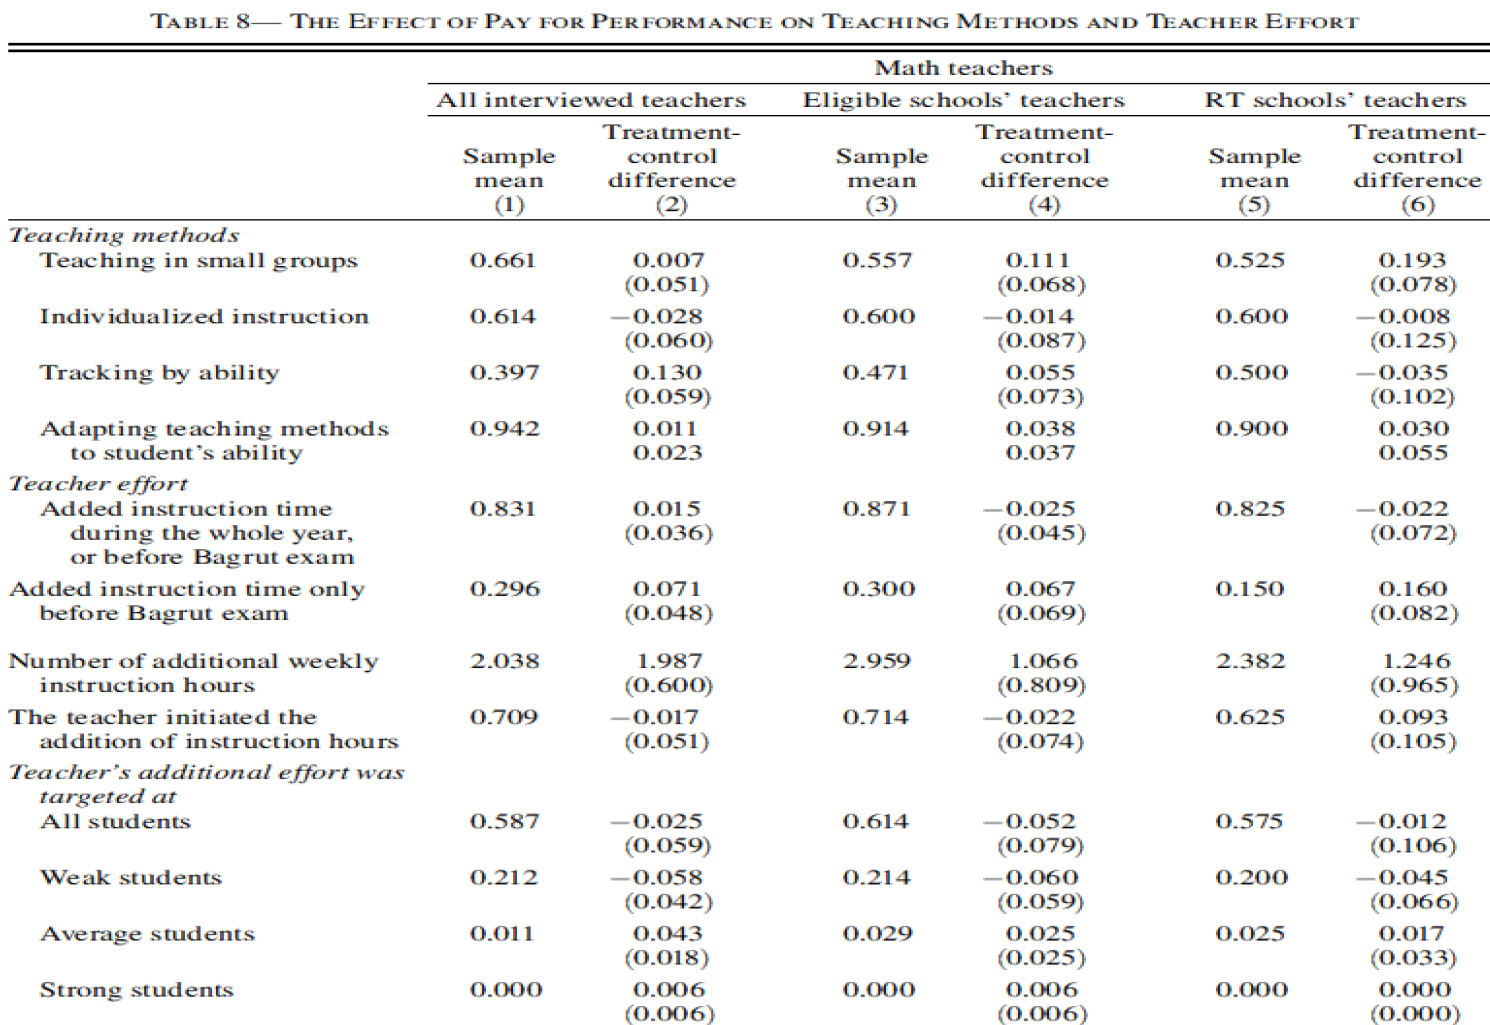
\includegraphics[width=4.5in]{images/ch10/10 lavy 2.png}
            \caption{Channels (\cite{lavy_performance_2009})}
        \end{figure}
        Interestingly, there's no obvious channels through which the improvement happens.